% Activate the following line by filling in the right side. If for example the name of the root file is Main.tex, write
% "...root = Main.tex" if the chapter file is in the same directory, and "...root = ../Main.tex" if the chapter is in a subdirectory.
 
%!TEX root =  

\chapter{Preliminary Study\label{prelim}}


\minitoc

This section describes the preliminary study phase of the project which is the time spent by the project team gaining insight into the problem the software system is to solve. For this project, the problem is very well defined from the customer's perspective, so little time is spent looking into similar products and various possible solutions to the overarching problem of computer aided privacy advice. A large portion of this time was spent on investigating the proposed solution and the technologies involved, that is Case Based Reasoning (CBR) and the technologies used by it. Another critical work laid down in this phase were choices with respect to project scope.

\section{Technology}


\subsection{Privacy technology}\label{privTech}
This section briefly describes the situation today with respect to Internet privacy tools and which needs the project seeks to address.

As discussed in T�ndel and Nyre (2010), there is a disproportion between the average Internet user's concern for privacy and the actual control he has over private information. While most websites provide a privacy policy, these tend to very long documents written in a obscure "legalesque" language, intended  for protecting the websites' interests than those of users. To aid this problem, machine readable standards such as P3P have been introduced. P3P seeks to compress the information contained in the privacy policy in an XML document that can be parsed and summarized by computer programs. 

The AT\&T \emph{Privacy Bird} is mentioned in T�ndel and Nyre (2010) as an example of current Internet privacy software. Privacy Bird can parse P3P documents and match a site's privacy policy with the user's preferences. The problem with this however, is that the user has to explicitly state his preferences, which is a rather time-consuming endeavor. The novel feature of this project is to introduce an intelligent system that \emph{learns} the user's preferences, seeking to limit the amount of user interference. This is to be achieved by the use of CBR agent, that can look at previous examples of user choices in similar situations. A particular advantage of the CBR approach is the feedback loop where the system can actually \emph{explain} its choice in terms of similar cases which sets CBR apart from alternative reasoning models such as artificial neural networks. It also allows for better tuning to user response in those cases that the user disagrees with the recommendation.

\subsection{Case Based Reasoning}
Being, the core part of the system to be developed, some time needed to be spent on looking into CBR. In vague terms, CBR is problem solving based on past solutions to previous problems. This approach is similar in many ways to the way humans solve problems, both as domain experts, and in their daily life. For instance, a software engineer, faced with a particular problem, may identify similarities to a problem he has previously solved, using for instance a factory design pattern, so he adopts this solution to the new problem with some modifications. Similarly, a NTNU student, hungry for a late night snack, recalling past experience with favorable opening hours and culinary excellency, heads off to Sesam.

\begin{figure}[htbp]
\begin{center}
\caption{A Simplified CBR Cycle.}
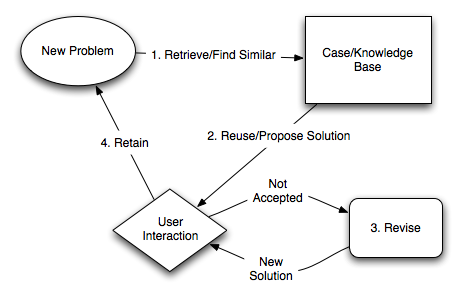
\includegraphics[width = .75\textwidth]{PrelimStudy/cbr}
\label{cbrCycle}
\end{center}
\end{figure}


For computer implementation, CBR is usually formalized in terms of a four step process:

\begin{itemize}
\item Retrieve: 
Given a new site, the agent will retrieve from its knowledge base, the set of cases deemed the most similar to the one at hand. This means, that if presented with the site Facebook, for instance, the agent finds Twitter, Google and LinkedIn to be the sites that have the most similar policy to Facebook.
\item Reuse: 
Look at the decisions made about the cases that were found and adapt this decision to the problem at hand. In this case, the agent needs to see if there are strong enough indications toward a particular behavior with respect to the type of site that is at hand. If for instance, the user has accepted the policies of all the similar sites found, he is also likely to accept that of Facebook.
\item Revise: 
Once a conclusion is reached, it is presented to the user (along with the background for why it is reached). The user may then choose to accept the conclusion, or to overrule it, providing the system with directions as to why it was wrong. This may in turn cause the agent to update its parameters accordingly. 
\item Retain: Finally, the new case is stored to the database along with the user�s decision as a reference for the next time the same site is opened, and as a case to employ when evaluating new sites.
\end{itemize}

As can be seen from this specification, CBR is a very generic approach, and several notions need to be defined before it can be implemented. For instance, we need to settle on a knowledge representation. For most CBR purposes, a frame based approach is taken. To store this knowledge representation, an appropriate database structure must be selected, and a routine for keeping this up to date must be established. Given a representation, one needs to define a notion of \emph{similarity} between cases, and an algorithm to do the actual retrieval. Usually, one would also like this algorithm to provide some measure of the certainty of the results as well.

While SINTEF has proposed some initial ideas for how these details can be implemented, they are very much open problems, and subject to empirical study to find an 'optimal' approach for the actual problem at hand.

\section{Project Scope}
The research nature of this project makes it a very open-ended one. The clearly most important part of the system envisioned by the customer is the CBR engine, that classifies websites based on the user's previous decisions. Implementing this is clearly necessary, regardless of which direction is followed and what limitations are made.

However, once the local CBR engine and auxiliary modules such as parsing P3P documents and so forth are in place, there are several directions that the project can take, and pursuing all of them is an unlikely scenario given the resource limitations. To some extent, the direction of the project also depends in a large extent on how well preliminary testing goes; that is, how well does the CBR system actually predict user preferences. Depending on the results of these tests, several possible directions were deemed possible:

\begin{enumerate}
\item Given test failure, making improvements to the algorithm, hereunder, the retrieval methods, the amount of data stored per case, the distance metric used to compare cases, and the weighting of the different features of a case/policy.
\item Extending the system by implementing the community portion/collaborative filtering part of the proposed system.
\item Given a test success, implementing a working browser plugin.
\item Closely related to the previous point, extending the system to work with other privacy policy standards.
\end{enumerate}

Direction 1 above takes the project from a system engineering direction more over to a scientific and statistical analysis type project, and while placing some emphasis on tuning the algorithms, this is not our primary focus\footnote{This would require gathering a dataset of some size as well as setting up testing scenarios, which not only requires a sophisticated statistics background, but also likely group of test users. It was decided that this should not be prioritized in a software engineering project of limited scope such as this.}. Item 3 relies heavily on the effectiveness of the algorithm and may require exactly the type of statistical analysis discussed. In agreement with the customer, it was therefore concluded that the collaborative filtering part was to be the second focus after the CBR part. 

\section{Development Model and Workflow}
Having briefly identified and outlined the project "flow", a development method or model must be chosen. A two-stage implementation process is envisioned; the first in which the core CBR is implemented. In the second part, the focus is on the community/CF portion. By thus splitting the work in two stages, time is made available for more thorough testing and reworking of the CBR portion, while work on the CF system, which is given a lower priority is pushed back. Given this project flow, we deemed that the work fits well within waterfall model framework. This is described in more detail in the next section. 

\begin{figure}[htbp]
\begin{center}
\caption{A standard waterfall process.}
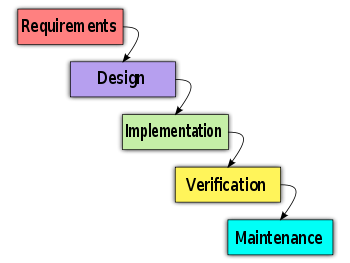
\includegraphics[width = .6\textwidth]{PrelimStudy/waterfall}
\label{waterfall}
\end{center}
\end{figure}

\subsection{The Waterfall Model}
The waterfall model describes the development process as a linear process that starts with planning and requirements specification, and flows sequentially through design, implementation and finally (in this case) testing as is illustrated in Figure~\ref{waterfall}. Arguments \emph{for} the waterfall approach is that it encourages rigorous planning and design, which means that inconsistencies and problems can be discovered earlier in the process, which is generally less costly than if they are discovered late, since this often means re-writing a large portion of code. 

Another advantage of the waterfall model, which relates directly to the nature of this particular project, is the focus on design. Since the software product to be delivered is a very early prototype that is to be used in further research, and likely to be further modified in the future, providing solid modularity and interfaces so as to allow code reuse is critical. Properly documenting the program structure, as encouraged by the waterfall model, will also be highly beneficial to anyone who is later to modify the program.

\begin{figure}[htbp]
\begin{center}
\caption{Development Model}
\includegraphics[width = 1.0\textwidth]{PrelimStudy/workflow}
\label{workflow}
\end{center}
\end{figure}

A common criticism raised against the waterflow model is that development rarely occurs in completely distinct stages; it is often hard to completely finish one phase of the project before moving on to the next. For instance, in many projects, requirements may be subject to uncertainty or change, so that design in turn must be altered. While recognizing this and other inherit weaknesses in the waterflow model, we think that for this project, requirements are quite clear, and since its scope is limited, a slightly modified waterfall model will still serve the project well. 

Among the modifications that we have made is, as indicated in Figure~\ref{workflow}, a slight overlap between the different phases. This is justified by the fact that some stages are not dependent entirely on the previous stage. For instance, given a detailed design, a test plan and testing procedures can be worked out independently, and testing of one module does not require the entire system to be integrated.